\cotefile{62}
\scanpage{2}
Courbes elliptiques
% archive sheet number: 1
\scanpage{4}
\uline{Modules des courbes elliptiques}

Soit $C$ une ``courbe elliptique'' homogène sur $S$ loc. noethérien. La section nulle $s$ définit un bon diviseur \inserted{$D$} sur $C$\inserted{ transversal aux fibres}, d'où un \deleted{fibré}\inserted{faisceau inv. $\underline L$}, dont les \inserted{germes de} sections sont des \deleted{\unsure{fonctions}} germes de fonctions sur $C$ (précisément celles qui sont des ``multiples'' de $D$). Notons que \deleted{$s^*(\underline L)\simeq$}, $C$ étant un schéma en groupes

\deleted{\uline{Proposition} 1 Les $L^n$ ($n\in\mathbb Z$) sont \unsure{cohomologiq$^{\rm t}$} plats en \unsure{ttes|tte} dimensions.}

\[
\underline{\mathfrak g}_{C/S}=f^{*}_{\deleted{\unsure{*}}}(s^*(\underline{\mathfrak g}_{C/S}))=f^*(\mathcal L_{C/S})\qquad [\mathcal L\unsure{.=|:=|=}\text{ faisceau de Lie}]
\]
\[
s^*(\underline L)\simeq s^*(\underline L\otimes_C\underline O_{S'})\simeq s^*(\underline N_{C/S'})\simeq s^*(\underline{\mathfrak g}_{C/S})\simeq\mathcal L
\]

Ce \unsure{faisceau|faisceaux} sera noté $\mathcal L_{\deleted{\unsure{s}}C/S}$ [``Lie'']. Donc
\[
s^*(\underline L^{\otimes n})\simeq\mathcal L_{C/S}^{\otimes n}
\]

On a une section \unsure{dedans|évidente} de $\underline L$, savoir la section constante $1$ de $\underline O_C$,
\[
\sigma:\underline O_C\longrightarrow\underline L\qquad \sigma\in\Gamma(C,\underline L)
\]
qui définit un homomorphisme (d'injection si on veut)
\[
\cdots\longrightarrow\underline L^{\otimes n}\longrightarrow\underline L^{\otimes(n+1)}
\longrightarrow\cdots\longrightarrow\underline L^{\otimes(n+\unsure{k|h|d})}\longrightarrow\cdots
\]
\margin{$\subset$ \unsure{faisc.|faisceau} des fonctions rationnelles relatives sur $C/S$}

donc \deleted{\unsure{un}} des homomorphismes
\[
\cdots\longrightarrow f_*(\underline L^{\otimes n})\longrightarrow f_*(\underline L^{\otimes(n+1)})\longrightarrow\cdots
\]
i.e.
\[
\cdots\longrightarrow\mathcal E_n\longrightarrow\mathcal E_{n+1}\longrightarrow\cdots
\]
en posant \(\mathcal E_n=f_*(\underline L^{\otimes n})\)
% archive sheet number: 3
\scanpage{5}
\uline{Proposition 1} Les faisceaux $\underline L^{\otimes n}$ sont coh. plats en ttes dimensions. Le faisceau $f_*(\underline L^{\otimes n})$ est localement libre, de rang $0$ si $\unsure{n|p}<0$, $1$ si $n=0$ ou $1$, $n\deleted{\unsure{-1}}$ si $n\geq1$. \deleted{\unsure{Le|$\underline L$}} Le faisceau $\underline L$ est ample, et de façon précise $\underline L^{\otimes n}$ est \deleted{\uline{très}} \uline{ample} \deleted{pour}\inserted{ssi} $n\geq1$, très ample ssi $n\geq3$

La formule de RR, où $g=1$, d'où $2g-2=0$, nous montre que \uline{tout faisceau} \deleted{loc libre} inversible sur $C$, de degré \inserted{relatif} $d\ne0$, est coh. plat, et que sa dimension est \deleted{\unsure{donné|donc}} nulle si $d<0$, et $d\deleted{\unsure{-(g-1)}}$ si $d\geq1$. Donc la première assertion est démontrée pour $n\ne0$, et pour $n=0$ elle est connue par ailleurs, car $\underline L^{\otimes n}=\underline O_C$.
% slanted
\margin{prop. préliminaire sur un faisceau inversible quelconque}

\inserted{On \deleted{\unsure{sait}} sait qu'un faisceau inv. sur $C$ de degré relatif $d$ est ample ssi $d\geq0$, donc $\underline L^{\otimes n}$ est ample ssi $n\geq1$.} \deleted{Et puisque le \unsure{$\underline L$ est de degré relatif $1>0$|$\underline L$ est de degré relatif $d>0$}, il est ample, pour voir s'il \unsure{donc} $\underline L^{\otimes n}$ est très ample pour $n>0$.}

Si $\underline L^{\otimes n}$ est très ample, on a $n\geq1$, d'ailleurs on ne peut avoir $n=1,2$ car alors $\mathbb P(f_*(L^{\otimes n}))$ est de dim relative $0$ ou $1$, donc $C$ ne peut s'y immerger (car il y serait isomorphe, absurde), donc il faut $n\geq3$. Celà suffit, car à cause de la platitude cohomologique, \deleted{et} \deleted{\unsure{est}} on est ramené au cas \deleted{où} $S=\unsure{\mathrm{Spec}|{\mathrm{Sp}}}\,k$, $k$ un corps\inserted{ alg. clos}. \deleted{Mais alors D'ailleurs, comme $\underline L$ est engendré loc$^{\rm t}$ par ses sections} Mais \deleted{alors} comme $3>(2g-2)+2=2g=2$, un raisonnement connu n'utilisant que RR donne le résultat.
% archive sheet number: 4
\scanpage{6}
\uline{Proposition} On a donc des \deleted{\unsure{homo|les}} inclusions
\[
\mathcal E_0\unsure{\subset|=}\mathcal E_1\subset\mathcal E_2\subset\mathcal E_3\subset\cdots
\]
les $\mathcal E_i$ \unsure{étant|sont} des faisceaux loc. libres de rang $i$ pour $i\geq1$. D'ailleurs
\[
\mathcal E_0=\underline O_S
\]

\uline{Proposition} 2 $\mathcal E_0=\mathcal E_1=\underline O_S$, d'autre part pour $i\leq j$ l'injection $\mathcal E_i\longrightarrow\mathcal E_j$ est \deleted{loc$^{\rm t}$.} universellement injective. \inserted{Soit} \deleted{Le faisceau} $\mathcal L_n\simeq\mathcal E_{\deleted{\unsure{n+1}}n}/\mathcal E_{n-1}$ \inserted{(pour $n\geq1$, \deleted{\unsure{$\underline O_S$}}, donc $\mathcal L_i$ est inv si $i\ne1$), alors on a des isomorphismes} \deleted{est isomorphe à $\mathcal L^{\deleted{\unsure{\otimes}}}$, et $\mathcal E_{n+1}/\mathcal E_n$ est isomorphe à $\mathcal L^{\otimes n}$.} $\mathcal L_n\otimes\mathcal L_m\simeq\mathcal L_{m+n}$ si $n,m\left|\begin{smallmatrix}\geq0\\\ne1\end{smallmatrix}\right.$, \inserted{correspondant} \deleted{faisant de} à \inserted{une structure} sur $\coprod_{n\geq0}\mathcal L_n$ \deleted{\unsure{une}} d'Algèbre graduée comm.

Pour la première assertion, à cause de la platitude coh., on est ramené au cas d'un corps, où c'est trivial car on a une injection.

Notons que $\mathcal E=\varinjlim\mathcal E_n=f_*(\varinjlim\underline L^{\otimes n})$ est une $\underline O_S$-\uline{algèbre}, dont la connaissance d'ailleurs implique la connaissance de $\underline\Gamma_*^{\unsure{\mathcal E|\xi}}(f,\underline L)=\coprod\mathcal E_n$, car $\mathcal E_m\times\mathcal E_n\longrightarrow\mathcal E_{m+n}$ est précisément induit par la multiplication de $\mathcal E$. On a, en passant au gradué associé à la filtration croissante donnée, une algèbre $\coprod_{n\geq0}\underline{\mathcal L}_n$, où les $\underline{\mathcal L}_n\simeq\mathcal E_n/\mathcal E_{n-1}$ pour $n\geq0$, en modifiant pour $n=0$ par $\underline O_S$. Il faut prouver que $\underline{\mathcal L}_n\otimes\underline{\mathcal L}_m\longrightarrow\underline{\mathcal L}_{n+m}$, $n,m\left|\begin{smallmatrix}>0\\\ne1\end{smallmatrix}\right.$, \deleted{$n,m$} \deleted{\unsure{est}} bien isom., ou encore surjectif, \deleted{et pour} Si $n$ ou $m=0$ \deleted{\unsure{réciproquement si $n$ et $m$ sont entiers}} c'est trivial, sinon on a $n,m\geq2$, et pour voir.
% archive sheet number: 5
\scanpage{7}
On est ramené à ceci

\uline{Corollaire} Si $n\geq2$, $\underline{\mathcal L}_n$ est isomorphe par les \unsure{hom induits} à $\underline{\mathcal L}_2^{\otimes n'}$ si $n$ pair, à $\underline{\mathcal L}_2^{\otimes n'}\otimes\underline{\mathcal L}_3$ si $n$ impair (où $n'\geq1$ dans le premier cas, $n'\geq0$ dans le deuxième).

Mais on a plutôt intérêt de procéder directement ainsi: On est ramené aussitôt par platitude coh. au cas où $S=\operatorname{Spec} k$, on peut alors un \unsure{élémt|élément} $f$ de $L_n$ non dans $L_{n-1}$, un $g$ de $L_m$ non dans $L_{m-1}$, donc $fg$ \deleted{\unsure{dans}} dans $L_{n+m}^{\unsure{\otimes}}$ mais manifestement pas dans $\unsure{L_{n-1}\otimes L_m|L_m\otimes L_n|L_{n+m-1}}$.

\uline{Corollaire} $\mathcal E_3$ engendre $\Gamma_*(f,\underline L)$

Considérons les opérations de $\underline{\mathfrak g}$ sur les germes de fonctions rationnelles sur $C$ [\unsure{restant|reste est} à définir], on constate que \deleted{$\underline{\mathfrak g}$} ces opérations induisent des hom
\[
\underline{\mathcal L}\otimes\underline{\mathcal L}_n\longrightarrow\underline{\mathcal L}_{n+1}\qquad n\geq2
\]

\uline{Proposition 3} \inserted{Soit $s\in S$, $p$ l'exp car. de $k(s)$.} L\deleted{es}'homomorphisme $\underline{\mathcal L}\otimes\underline{\mathcal L}_n\longrightarrow\underline{\mathcal L}_{n+1}$ est un \uline{isomorphisme} (\unsure{vu|en|voir} \deleted{\unsure{au|ordre}} sur $c$ \unsure{point|près}) ssi $p$ est premier à $n$

On est ramené au cas où $S=\operatorname{Spec} k$, et alors c'est une vérification locale: si $D$ est une \deleted{diff.} dérivation rég. non nulle en un pt\inserted{ $x\in C$}, et si $f\ne0$ sur $C$ a en $x$ un pôle d'ordre $n$,
% archive sheet number: 6
\scanpage{8}
\deleted{non divisible par $p$} alors \deleted{$Df$} $Df$ a en $x$ un pôle d'ordre au plus $n+1$, et égal à $n+1$ ssi $p\nmid n$.

\deleted{\uline{Corollaire 1} Si $k(s)$ est de car nulle, alors $\underline{\mathcal L}\otimes\underline{\mathcal L}_n\simeq\underline{\mathcal L}_{n+1}$ pour tt $n\geq2$, donc \deleted{$\underline{\mathcal L}_3\otimes\mathcal L\otimes\underline{\mathcal L}_2,\mathcal L_4$} \inserted{$\mathcal L_4\simeq\mathcal L_2\otimes\mathcal L^2$} $\mathcal L_n\simeq\mathcal L^{n-2}\otimes\mathcal L_2$, \deleted{donc} pour $n\geq2$, \deleted{\unsure{donc on} $\mathcal L_2\unsure{\simeq}$}}

\deleted{\uline{Corollaire} 2 Si $k(s)$ est de car $p\ne2$, alors \deleted{$\mathcal L_3\unsure{\otimes}\simeq\mathcal L_2\otimes\mathcal L$}, $\underline{\mathcal L}_4\simeq\underline{\mathcal L}_3\otimes\mathcal L$, $\mathcal L_6\simeq\underline{\mathcal L}_5\otimes\underline{\mathcal L}$ etc. $[\underline{\mathcal L}_{2n}=\underline{\mathcal L}_{2n-1}\otimes\mathcal L\ \text{si }n\geq2]$, enfin
\[
\mathcal L_2^{\deleted{\unsure{2}}}\simeq\mathcal L^{\otimes2}
\]}

\uline{Corollaire} Si $S$ est de car $p>0$ (i.e. $p\underline O_S=0$) et si $n$ est un multiple de la caractéristique, alors $\mathcal L\otimes\underline{\mathcal L}_n\longrightarrow\underline{\mathcal L}_{n+1}$ est \uline{nul}.

\deleted{\unsure{Propo|Prop|Prop.}} Considérons la suite exacte canonique
\[
\unsure{0|\cdot}\longrightarrow\underline L^{\otimes n}\longrightarrow\underline L^{\otimes n+1}\longrightarrow
(\underline{\mathfrak g}_{C/S}^{\otimes(n+1)})\otimes_{\underline O_{\unsure{C|S}}}\underline O_{S'}\longrightarrow0
\]
on en conclut la suite exacte
\[
0\longrightarrow\mathcal E_n\longrightarrow\mathcal E_{n+1}\longrightarrow\mathcal L^{\otimes(n+1)}\longrightarrow
\underset{\substack{\Vert\\0\ \text{si }n\geq1}}{\deleted{\unsure{R}}R^{1}(f,\underline L^{\otimes n})}
\]
d'où
\[
\boxed{\mathcal L_{n+1}\simeq\mathcal L^{\otimes(n+1)}\qquad n\geq2}
\]
% slanted
\margin{intervertir avec la prop. 2}
et la multiplication dont il est question dans prop. 2 n'est autre que la multiplication triviale pour cette forme des $\mathcal L_n$, $n\geq2$
% archive sheet number: 7
\scanpage{9}
Considérons maintenant l'immersion projective
\[
C\longrightarrow P(\mathcal E_3)
\]
définie par $L^{\otimes3}$ en vertu de prop. 1. Alors, $C$ devient un diviseur positif sur $P(\mathcal E_3)$ simple sur $S$, \inserted{de degré relatif 3,} il est donc défini par une \deleted{\unsure{élément|diviseur}} \inserted{section sur $S$} de l'espace des 3-formes
\[
\Phi_3(P(\mathcal E_3))\simeq P(\mathrm{Symm}_3(\check{\mathcal E}_3)).
\]
\deleted{De plus, comme}

\deleted{\uline{Supposons} que l'on se soit donné une trivialisation}

Considérons la section $s$ de $P(\mathcal E_3)$ et la \deleted{``droite'' \unsure{sur espace de dim 1|sous espace de dim 1}} \inserted{droite relative $D$} de $P(\mathcal E_3)$ définis comme $P(\mathcal E_3/\mathcal E_2)$ et $P(\mathcal E_3/\mathcal E_1)$, alors on constate que $s$ est une section de $C$, et que $D$ est une ``tangente d'inflexion'' ..... peu importe.

\figure{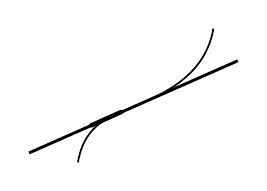
\begin{tikzpicture}[x=1cm,y=1cm]
\draw[line width=1.05pt] (0,0.12) -- (2.65,1.29);
\draw[line width=1.6pt,line cap=round] (.79,.47) -- (1.17,.64);
\draw[line width=.6pt] (.62,0) .. controls (.72,.60) and (1.20,.61) .. (1.53,.80) .. controls (1.98,1.00) and (2.27,1.28) .. (2.34,1.70);
\end{tikzpicture}}

Considérons une \deleted{trivialisation} \inserted{base de $\mathcal E_3$ compatible avec} \unsure{du clivage|des clivages} $0\subset\mathcal E_1\subset\mathcal E_2\subset\mathcal E_3$ de $\mathcal E_3$, \inserted{et commençant par $1_S\in\Gamma(S,\underline O_S)$,} [elle ``dépend en $(3+3-1)\inserted{{}=5}$ paramètres''], \deleted{par des coordonnées $\unsure{z,y,x|x,y,x}$} \inserted{i.e. une base $1,y,x$}

\[
\left(\begin{array}{ccc}
1&\unsure{\alpha|a}&\beta\\
\diagdown&\unsure{\mu|h}&\gamma\\
&&\unsure{\nu|v}
\end{array}\right)
\]

\deleted{Alors la forme $\varphi$ (définie à \deleted{\unsure{l'ordre}} \inserted{multiplication près par une} unité) prend la forme [où on remplace $z$ par $1$]
\[
a x^{\deleted{\unsure{3|2}}\unsure{2|3}}+b y^3+cxy+d y^2+ex+fy+g=0
\]
\unsure{$x^3y^2$|$y^3x^2$} où $y$ \unsure{désigne un suppl. de $\mathcal E_1$ dans $\mathcal E_2$} \inserted{\unsure{et $x$ de $\mathcal E_2$ dans $\mathcal E_3$}}}
% archive sheet number: 8
\scanpage{10}
\deleted{qui est aussi la relation (unique, \inserted{à unité près,} on la vérifie aussi bien à priori) vérifiée par} Puisque $1,y,x,y^2,xy,y^3$ forment une base de $\mathcal E_6$ (adaptée à sa filtration) on aura donc une équation
\[
\varphi(x,y)=\boxed{x^2+ay^3+bxy+cy^2+dx+ey+f=0}
\]

\[
\Delta(a,b,c,d,e,f)\in L^{\otimes12}
\]

qui est d'ailleurs une équation \unsure{valable|soluble} dans $\mathcal E_6$ considéré comme composante de $\Gamma_{*\mathrm{\unsure{rel}}}(f,\underline L^{\otimes})\simeq\coprod_{i\geq0}\mathcal E_{3i}$, satisfaite entre les sections $x,y$ de $\mathcal E_3$ \deleted{\unsure{et $x$ de $\mathcal E_3$|$x_1,x_2$} \unsure{$y$ de $\mathcal E_2$|$x_3$}}, \inserted{à valeurs en $\mathcal E_{\unsure{3.3|9}}$ \deleted{\unsure{resp.}}} \deleted{Cette équation} Si on désigne par $z$ la section $1$ de $\mathcal E_0,=\mathcal E_1\subset\mathcal E_3$, et qu'on \deleted{\unsure{la}} écrit \inserted{\unsure{une|ici} \deleted{la} équation} sous la forme
\[
\Phi(x,y,z)=x^2z+ay^3\deleted{z}+bxyz+cy^2z+dxz^2+fz^3=0
\]
% slanted
\margin{détailler, et éventuellement généraliser}
on \uline{constate alors} que $\Phi$ est la forme de degré 3 qui définit \deleted{\unsure{alors}} $C$ dans $P(\mathcal E_3)\simeq\mathbb P^3_S$. En effet si $\Phi'$ est la forme qui définit $C$, alors $\Phi$ est \uline{un multiple de $\Phi'$} et \deleted{\unsure{d'un coef.}} c'est un multiple par quelque chose qui est inversible, puisque $\Phi$ est ``non nulle'' en tt pt de $S$ --- un de ses coefficients c'est 1 ---.

% slanted
\margin{préciser ce pt cf intersections complètes}
% archive sheet number: 9
\scanpage{11}
Réciproquement, partons d'une équation comme dessus, où les \deleted{$a$} \inserted{coeff. $a,b$ ---} sont des sections de $\underline O_S$. On sait qu'\deleted{\unsure{elle|ce}} \inserted{une telle équation} définit un diviseur relatif \inserted{positif} de $\mathbb P^2_S/S$, soit $C$. Il reste à écrire que c'est là une \uline{courbe simple} sur $S$. On sait qu'il f et s pour celà que le discriminant de la forme
\[
\delta(a,b,c,d,e,f)
\]
soit une \uline{unité} partout. Ici le discriminant s'explicite : ---

On a obtenu en résumé

\uline{Proposition} La donnée d'une courbe elliptique sur $S$, \deleted{\unsure{avec}} \inserted{munie} d'une \deleted{``base adaptée''} \inserted{``base spéciale''} de $\mathcal E_3(C/S)$, \deleted{``\unsure{adaptée}''} est équival\deleted{\unsure{ents}}ente à la donnée de sections $a,b,c,d,e,f$ de $\underline O_S$ satisfaisant à $\delta(a,b,c\unsure{,|+}d,e,f)=0$, cette correspondance est compatible avec l'image inverse.

On déduit de ceci : Considérons le schéma affine de type fini sur $\mathbb Z$
\[
M=\mathrm{Spec}\bigl(\mathbb Z[A,B,C,D,E,F][\delta^{-1}]\bigr)
\]
qui est un ouvert affine de $\mathrm{Spec}\,\mathbb Z[A,B,C,D,E,F]\simeq\mathbb E^6_{\mathbb Z}$. \deleted{Faisons opérer \unsure{dans ce|dessus}}
% archive sheet number: 10
\scanpage{12}
\deleted{puis schéma de groupes $G$, de type fini sur $\mathbb Z$, qui \deleted{\unsure{repr.}} est représenté matriciellement par} \unsure{$\mathcal G$|Rq.|$\mathbb E_{\mathbb Z}$|$\underline O_{\mathbb Z}$}. Considérons le sschéma en groupes de $\unsure{\mathrm{Gl}(3)|\mathrm{Gl}(n)}_{\mathbb Z}$ qui correspond aux matrices de la forme
\[
\begin{pmatrix}1&\alpha&\gamma\\0&\lambda&\beta\\0&0&\mu\end{pmatrix}
\]
(avec $\lambda\mu$ une unité bien sur), \inserted{il opère sur $M$} de la façon évidente qui consiste à interpréter $ABCDEF$ comme coeff. d'une forme
\[
\deleted{\unsure{X^2+AXY^2|X^3+AXY^2}} \quad X^2+AY^3+BXY^2+CY^2+DX+EY+F
\]
et en faisant sur $X,Y$, la substitution affine
\[
\deleted{X}Y'=\lambda\deleted{X}Y+\alpha,\quad X'=\mu X+\beta Y+\gamma
\]
[on peut aussi dire --- ce sera plus clair, que $G$ opère dans le vectoriel $\mathbb E_3$, donc dans $\Phi_3(\mathbb E_3)$, et qu'il laisse invariant le sous-\deleted{\unsure{espace}}\inserted{module loc. libre} de \deleted{\unsure{formes}} rang 6 des formes qui sont de la forme dite, d'où les opérations de $G$ sur $M$.

\margin{\uuline{Prop}}

Alors le foncteur qui à tt $S$ en-dessous associe \inserted{l'\unsure{ens|ens.} des classes à isom près} des courbes elliptiques ``structurées'' comme dessus sur $S$, est \uline{représentable} par $M$. De plus, \deleted{\unsure{p}}pour que deux élém de
% archive sheet number: 11
\scanpage{13}
$M(S)$ définissent des courbes elliptiques isomorphes (\unsure{non|bien} structurées) il f et s que \deleted{\unsure{elles}} ils soient congrus par une opération de $G(S)$, où \inserted{$G$ est un groupe simple sur $S$.} Enfin, pour tte courbe elliptique $C$ sur $S$, il existe une extension \deleted{fidt plate} \inserted{simple surj. de type fini} $S'$ de $S$ [savoir le fibré principal associé à $\mathcal E_3$ pour le clivage qu'on a mis sur $\mathcal E_3$] tel que \deleted{\unsure{sur}} $C\times_S S'$ ``provienne'' d'un élément de $M(S')$.

Ainsi, avec une terminologie qui court, le foncteur $F$ : ``classes à isom près de courbes elliptiques sur $S$'' est \deleted{\unsure{fppf}}-$\mathcal D$-représentable, où $D$ désigne la catégorie des morphismes simples surjectifs. Si ce n'était que pour obtenir celà d'ailleurs on n'aurait pas à se donner tant de mal, \uline{car} \unsure{là|de} on a un raisonnement général qui le donne pour les courbes de genre $g$ \unsure{quelc} (le groupe triangulaire remplacé par un groupe projectif ---).
% archive sheet number: 12
\scanpage{14}
Une normalisation \deleted{\unsure{est}} un peu plus poussée est obtenue ainsi : On se donne une trivialisation de $\mathcal L$ par une section partout non nulle $D$ de $\mathcal L$, [dérivation invariante], on choisit alors la base $1,x,y$, de $\mathcal E_3$ de façon que l'image de $y$ dans $\mathcal L_2$ soit $i_2(D)$, celle de $x$ dans $\mathcal L_3$ soit $i_3(D)$. \deleted{\unsure{Celà|Cet}}

\deleted{$[$} i.e. on prend comme structure auxiliaire la donnée d'un $\mathcal L$ \inserted{inv.}, d'un $\mathcal E$ loc. libre de rang 3, muni d'un \unsure{splitting|splittage} où les facteurs successifs sont munis un isom avec $\mathcal L^0,\mathcal L^2,\mathcal L^3$ respectivem. Le groupe d'automorphismes de cette structure est \deleted{formé} \unsure{le|donc le} sous-groupe de $G_m\times\mathrm{Gl}(3)$, formé des \deleted{\unsure{triplets}} \inserted{couples} de la forme
\[
\begin{aligned}
\left(\lambda,\begin{pmatrix}1&\alpha&\beta\\0&\lambda^2&\gamma\\0&0&\lambda^3\end{pmatrix}\right)
&\qquad \lambda\in\Gamma(G_{m_S}/S)=\Gamma(S,\underline O_S^{\unsure{*|\times}})\\
&\qquad \alpha,\beta,\gamma\in\Gamma(S,\underline O_S)
\end{aligned}
\]

\deleted{La fixation de la structure ainsi conduit à une équation} Isomorphe \deleted{\unsure{i.e.}} au sous-groupe du \deleted{\unsure{précédent}} \inserted{groupe plus haut}
\[
\begin{pmatrix}1&\alpha&\beta\\0&\lambda&\gamma\\0&0&\mu\end{pmatrix}
\quad\text{pour}\quad \lambda=\left(\frac{\mu}{\lambda}\right)^2,\quad \mu=\left(\frac{\mu}{\lambda}\right)^3
\quad\text{i.e.}\quad \boxed{\mu^2-\lambda^3=0}.
\]

L'équation de $C$ pour une telle base \deleted{prend alors la forme} [caractérisée par la condition $\underline{x^2-y^3\in\mathcal E_5}$] prend la forme
\[
x^2-y^3+bxy+cy^2+dx+ey+f=0
\]
[i.e. on prend $a=-1$ en l'équation plus haut]
\[
\boxed{\delta(b,c,d,e,f)\text{ une unité}}
\]
% archive sheet number: 13
\scanpage{15}
Il ne semble pas qu'on puisse obtenir des normalisations locales sans \deleted{\unsure{hyp}} restriction de car. qui fasse intervenir moins de paramètres, [si on veut qu'elle soit subordonnée à la descente \deleted{\unsure{si|sur}} par morphismes plats, ou même simples]. Si on admet des ext. de base finies et plates, on peut pousser la normalisation plus loin en exigeant que \deleted{\unsure{le}} $\delta(b,c,d,e,f)=1$ i.e. \inserted{(intrinsèquement)} se bornant à des trivialisations de $L$ \deleted{compatibles} définies par des sections $\lambda$ dont la puissance $12$.\textsuperscript{ème} (ou est-ce $24$.\textsuperscript{ème}) est \inserted{$\delta^{-1}$, où $\delta$ est} le discriminant. On a \deleted{\unsure{en car.}} alors des \deleted{\unsure{plus}} normalisations plus poussées en car $\ne2$, puis en car. $\ne3$, puis \unsure{on vieillira|on veillera}.
% archive sheet number: 14
\scanpage{16}
Transformant l'équation
\[
x^2=y^3+axy+by^2+cx+dy+e
\]
par $s$, \deleted{et} se rappellant que $sx=-x$, $sy=y$, on trouve
\[
x^2=y^3\deleted{\unsure{+}}-axy+by^2-cx+dy+e
\]
et en comparant on trouve $a=c=0$, donc l'équation s'écrit maintenant sous la forme
\[
\boxed{x^2=y^3+ay^2+by+c}
\]
avec comme condition $\delta(a,b,c)\ne0$, qui ici ne fait qu'exprimer que les solutions de $P(y)=y^3+ay^{\unsure{2|1}}+by+c$ sont distinctes en tt pt de $S$.

Géométriquement, \deleted{\unsure{la situ.}} l'équation s'interprète ainsi : Le quotient $C/\mathbb Z_{/2}$ est un schéma de Brauer-Severi \inserted{$P$} sur $S$, muni d'une section marquée (correspondant à la section nulle de $C$ sur $S$), donc \deleted{s'identifie} \deleted{est isomorphe} \inserted{canoniquement} à un espace principal homogène sous un \deleted{fibré \unsure{qui est loc libre}} \deleted{\unsure{faisceau inversible}} fibré vectoriel \deleted{\unsure{homogène}} \inserted{inversible} [il correspond : $L^{\otimes2}$]
% slanted
\margin{\unsure{précisons|préciser|provisoire}}

$C$ est ramifiée \deleted{\unsure{et}} au dessus d'un diviseur relatif \inserted{de $P/S$} étale sur $S$, qui se décompose en la section à l'infini, et en un diviseur \deleted{\unsure{de}} relatif \inserted{de $\unsure{\mathring P|\dot P|P}/S$} étale sur $S$, \deleted{\unsure{et en fait de}} de \deleted{$\unsure{\mathcal E}$} $\underline V(L^{\otimes2})/S$ étale sur $S$, de degré relatif 3.
% archive sheet number: 15
\scanpage{17}
\deleted{Supposons \unsure{quelque soit|quelles soient|qu'on soit} les corps résiduels de}

Notons qu'il y a dans $C$ un $S$-automorphisme canonique de symétrie, car $C$ est un schéma abélien sur $S$. Cet automorphisme \inserted{est d'ordre 2, il} opère sur les $\mathcal E_i$ [de façon compatible avec les structures multiplicatives \inserted{et les opérations de $\mathcal L$ sur $\mathcal E_\infty$}] et induit sur $\mathcal L$ le changt de signe. \deleted{Il en résulte aussitôt qu'il opère \unsure{trivialemt} dans $\mathcal E_2$. Et il y aura un \unsure{supplémentaire vers $\mathcal E_1$},} \deleted{Si les caractéristiques résiduelles de $S$ sont $\ne2$, on en conclut} Supposons les car. résiduelles de $S$ $\ne2$. Alors

\deleted{1) Il existe un supplémentaire unique de $\mathcal E_1$ dans $\mathcal E_2$ \unsure{stable} \unsure{qui sur lequel} $s$ opère}

% slanted
\margin{N.B. la \unsure{considération|construction|condition} de $C\to P(\mathcal E_2)$ et de la différent. de ce morphisme nous donne (sans restriction en car) un morphisme $\mathcal L^{\otimes3}\overset{\unsure{\sim}}{\longrightarrow}\mathcal E_3$ compatible avec les automorphismes (car fonctoriel en $S$).}

$s$ opère trivialemt dans $\mathcal E_2$ [c'est même sans la restriction qu'on vient de faire, on le verra], et il existe un supplémentaire unique \inserted{$L_3$} de $\mathcal E_2$ dans $\mathcal E_3$ où $s$ opère par symétrie, \deleted{\unsure{lequel}} qui est aussi égal à : $\mathcal L\cdot\mathcal E_2$, on le note $L_3$.

\deleted{Alors $L_3^{\otimes2}$ est un supplémentaire de $\mathcal E_5$ dans $\mathcal E_6$, soit $L_6$. A condition} On peut donc normaliser encore plus les bases admissibles de $\mathcal E_3$, en exigeant que $x$ soit une base de $\mathcal E_3$ ; donc le groupe des changemts de base admis est ceux de la forme
\[
\begin{pmatrix}1&\alpha&0\\0&\lambda^2&0\\0&0&\lambda^3\end{pmatrix}
\quad\text{i.e.}\quad
\begin{pmatrix}1&\unsure{\alpha|a}&0\\0&u&0\\0&0&v\end{pmatrix}
\quad\text{avec}\quad\deleted{\unsure{\lambda\lambda|\lambda}}u^3-v^2=0.
\]
Ce n'est autre que le \uline{groupe affine à 1 variable}.

Quelle est la normalisation correspondante de l'équation de $C$ ?
% archive sheet number: 16
\scanpage{19}
\deleted{$\unsure{7|j|\mathbb Z}$} $b$\qquad $j$ et $j-1$ \unsure{unité|unités}

Cas $A$ local \uline{\unsure{normal ?}}
\[
\left\{\begin{aligned}
&j\text{ une unité, pas }j-1,\ (\text{pas idt nul})&
(1\unsure{-|+}j^{-1})^2\in A^6 A^{\unsure{*}}\\
&j-1\text{ une unité, } j\text{ pas (pas idt nul)}&
\left(\frac{\unsure{1|j}}{j-1}\right)^3\in A^6 A^*
\end{aligned}\right.
\]

% slanted
\margin{\uline{à vérifier} \uline{géométriquemt}}

\diagram{\begin{tikzcd}[ampersand replacement=\&,column sep=small]
{\text{Ext. Kummérienne du groupe }\mathbb Z/3}\arrow[r,leftrightarrow]\&j\equiv1\\
{\text{Ext. Kummérienne du groupe }\mathbb Z/2}\arrow[r,leftrightarrow]\&j\equiv0
\end{tikzcd}}

\[
\begin{aligned}
b^3=0,\ c\text{ inversible}\quad /\!/ &\ \text{si }\deleted{\unsure{a}} A\text{ sans élément nilpotents, alors l'invariant}\\
&\ \text{est }c\in A^*/A^{*(3)}\\
c^2=0,\ b\text{ inversible}\quad /\!/ &\ \text{si } A\ \text{ss élémt nilpotts,}\\
&\ \text{alors l'invariant est }b\in A^*/A^{*(2)}
\end{aligned}
\]

$1-$

\figure{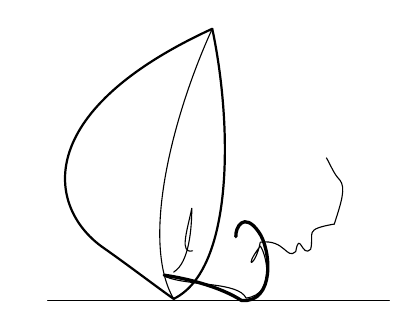
\begin{tikzpicture}[x=1cm,y=1cm,line cap=round,line join=round]
\draw[thin] (-.12,0)--(4.22,0);
\draw[thick] (1.97,3.45).. controls (-.36,2.38) and (-.12,1.15)..(.60,.66).. controls (.90,.45) and (1.28,.16)..(1.48,.02);
\draw (1.97,3.45).. controls (1.48,2.38) and (1.05,.76)..(1.48,.02);
\draw[thick] (1.97,3.45).. controls (2.22,2.28) and (2.26,.40)..(1.48,.02);
\draw[very thick] (1.36,.32).. controls (1.65,.28) and (2.08,.17)..(2.34,.00).. controls (2.77,-.04) and (2.72,.65)..(2.56,.87).. controls (2.37,1.14) and (2.26,.92)..(2.27,.81);
\draw (1.38,.30).. controls (1.68,.18) and (2.30,.24)..(2.40,.03).. controls (2.79,.08) and (2.65,.60)..(2.58,.69).. controls (2.35,.39) and (2.52,.42)..(2.58,.74).. controls (2.90,.78) and (2.91,.51)..(3.03,.62).. controls (3.08,.90) and (3.11,.53)..(3.22,.65).. controls (3.27,.86) and (3.12,.90)..(3.52,.97);
\draw (3.52,.97).. controls (3.61,1.25) and (3.67,1.43)..(3.59,1.53).. controls (3.51,1.61) and (3.47,1.73)..(3.42,1.81);
\draw (1.48,.36).. controls (1.68,.48) and (1.71,.93)..(1.71,1.17).. controls (1.65,.88) and (1.55,.59)..(1.72,.63);
\end{tikzpicture}}

\[
\begin{aligned}
\deleted{\unsure{j-1|j\equiv1}} \quad \left(\frac{t}{t-1}\right)^3 &\in O^6O^* &\quad&\text{\uline{marche pas}}\\
\left(\frac{t-1}{t}\right)^2 &\in O^6 O^{\unsure{*|\times}} &&\text{''}\qquad \sqrt[6]{\frac{t\deleted{\unsure{-1}}}{t-1}}
\end{aligned}
\]

\[
\sqrt[2]{\frac{t}{t-1}}\qquad \sqrt[3]{\frac{t-1}{t}}\qquad 1/2\qquad 1/3
\]

\figure{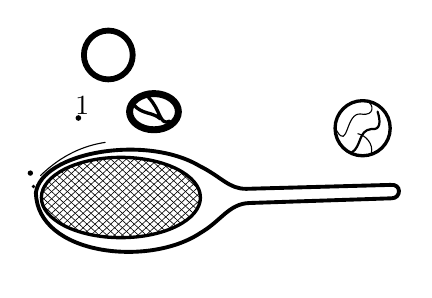
\begin{tikzpicture}[x=1cm,y=1cm,line cap=round,line join=round]
% crop-candidate: scan 19
\draw[line width=2.1pt] (1.02,2.66) circle (.31);
\draw[line width=2.5pt] (1.60,1.94) ellipse (.31 and .23);
\draw[very thick] (1.34,2.03).. controls (1.45,1.90) and (1.58,1.94)..(1.68,1.85) (1.53,2.12).. controls (1.68,1.98) and (1.67,1.75)..(1.80,1.82);
\draw[line width=1.2pt] (4.25,1.73) circle (.35);
\draw (3.92,1.70).. controls (4.07,1.44) and (4.03,1.94)..(4.23,1.91).. controls (4.41,1.88) and (4.39,2.04)..(4.31,2.07);
\draw[thick] (4.11,1.42).. controls (4.24,1.50) and (4.19,1.70)..(4.36,1.72).. controls (4.48,1.70) and (4.48,1.82)..(4.44,1.94);
\draw (4.19,1.66).. controls (4.29,1.64) and (4.39,1.53)..(4.36,1.41);
\draw[line width=1.4pt] (.10,.91).. controls (.17,1.42) and (1.49,1.66)..(2.18,1.25).. controls (2.46,1.11) and (2.55,.96)..(2.77,.96)--(4.60,1.01).. controls (4.75,1.03) and (4.74,.84)..(4.62,.84)--(2.81,.78).. controls (2.55,.77) and (2.45,.55)..(2.19,.40).. controls (1.53,-.04) and (.12,.12)..(.10,.91);
\draw[very thick] (1.18,.85) ellipse (1.01 and .51);
\begin{scope}
\clip (1.18,.85) ellipse (1.01 and .51);
\foreach \x in {-1,-.90,...,3.4}{\draw[line width=.22pt] (\x,.19)--++(1.36,1.25);\draw[line width=.22pt] (\x,.19)--++(-1.36,1.25);}
\end{scope}
\draw (.16,1.13).. controls (.44,1.40) and (.72,1.51)..(.98,1.55);
\fill (.03,1.16) circle (.034) (.07,.99) circle (.024) (.64,1.86) circle (.036);
\node at (.69,2.02) {$1$};
\end{tikzpicture}}

\[
\lambda^{3/6}\cdot\lambda^{\unsure{-2/6|-1/6}}=\lambda^{1/6}
\qquad \frac{-27c^{\unsure{2}}}{b^3-27c^2}=j
\]
\[
\deleted{\unsure{\sqrt[6]{t}}}\qquad s^6=\frac{t}{t-1}\qquad \frac{b^3}{c^2}=j\qquad 27c^2(j-1)=b^3j
\]

\[
\begin{array}{ccc}L&L^2&L^3\\&b&c\end{array}
\qquad
\begin{aligned} b^{\deleted{\unsure{3}}}&=27\frac{j-1}{j}\\ c&=27\frac{j-1}{j}\end{aligned}
\qquad \boxed{\frac{b^3}{c^2}=27\frac{j-1}{j}}
\]

% slanted
\margin{\unsure{$L_m-L-$}}

\figure{
\begin{tikzpicture}[x=1cm,y=1cm,line cap=round,line join=round]
\draw[thick] (.00,.67).. controls (.02,1.51) and (1.05,1.62)..(1.40,.99).. controls (1.71,.94) and (2.66,1.13)..(3.01,1.08).. controls (3.21,1.06) and (3.20,.82)..(3.01,.82).. controls (2.52,.91) and (1.75,.79)..(1.41,.75).. controls (1.11,.18) and (.74,-.11)..(.28,.19).. controls (.08,.34) and (-.03,.48)..(.00,.67);
\draw (.09,.42).. controls (.34,.03) and (.92,.00)..(1.17,.26) (2.88,.85).. controls (3.12,.87) and (3.15,1.01)..(2.96,1.05);
\fill (-.18,-.13).. controls (.04,-.14) and (.12,-.06)..(.31,-.08).. controls (.21,-.17) and (.01,-.23)..(-.18,-.13);
\end{tikzpicture}}

\[
\boxed{x^3+27\frac{\unsure{j|t}-1}{j}(x+1)=0}
\]

\deleted{$\unsure{\mathrm{Hom}(E,}$}\quad $f_*(\check E)$

\diagram{\begin{tikzcd}[ampersand replacement=\&]
\underline{\mathrm{Hom}}_O(E,\underline O)\\
\mathrm{Hom}_{\underline A}(E,\underline A)\times\mathrm{Hom}_{\underline O}(\underline A,\underline O)\arrow[u]
\end{tikzcd}}
% archive sheet number: 18
